\subsection{Instantaneous 2D sphere}\label{sec:ist_sphere}
The domain is a unit square with gravity $\bm{g}=(0,-1)$. The fluid has constant density and viscosity ($\rho_f=1$ and $\eta_f=1$). The sphere is in the middle
of the domain with a radius R = 0.123456798 and has constant density and viscosity ($\rho_s=10^{-2}+\rho_f$ and $\eta_s=10^3 \cdot \eta_f$).
We distinguish three different types of velocity boundary conditions:
\begin{enumerate}
\item FS: free slip conditions on all sides.
\item NS: no slip conditions on all sides.
\item OT: free slip conditions on the sides and the bottom, and open boundary at the top.
\end{enumerate}
All three cases are performed for different grid resolutions, between $16 \times16$ and $512\times 512$ elements with 50 randomly distributed markers per element,
and different average schemes for the viscosity (harmonic, geometric and arithmetic). The velocity in the centre of the sphere $\bm{v}(0.5;0.5)$, minimum and
maximum velocities ($u_{min}$, $u_{max}$, $v_{min}$, $v_{max}$) and pressures ($p_{min}$, $p_{max}$) on the entire domain, $v_{\textrm{rms}}$ and average pressure on the
entire domain ($p_{avg}$) are compared with solutions generated by ASPECT \citep{Kronbichler2012,Heister2017,Bangerth2020,Bangerth2020a} and all results
can be found at \url{https://github.com/cedrict/fieldstone/tree/master/images/stokes_sphere2D} and 
\url{https://github.com/aleregorda/Benchmarks/tree/main/Momentum_equation/Instantaneous_2D_Sphere}. Results in terms of the $v_{\textrm{rms}}$ for NS model 
are also shown in Fig. \ref{fig:inst_sphere}.

\begin{figure}
\centering
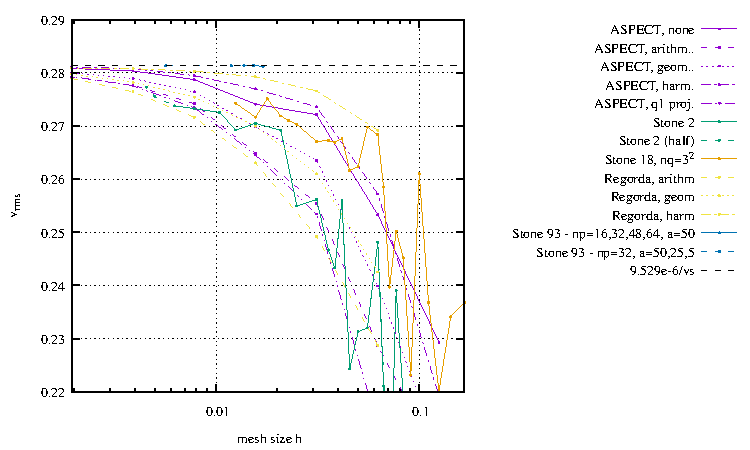
\includegraphics[width=400px]{./Figures/vrms_NS.pdf}
\caption{$v_{\textrm{rms}}$ as function of element size for the instantaneous 2D sphere experiment in case of no slip boundary conditions and with different average
schemes for the viscosity. Results are compared with results obtained by other numerical codes.}
\label{fig:inst_sphere}
\end{figure}